% Appendix_I.tex
% Placement: copy this file to `appendix/Appendix_I.tex` in the paper repo.
% Expected figure location: the paper root's `figures/` directory.
% The main paper already defines \graphicspath{{figures/}}, so the figure
% filenames below are given without a directory prefix.

\section{Experimental Results}
\label{app:experiments}

\setcounter{figure}{0}
\renewcommand{\thefigure}{\thesection.\arabic{figure}}

This appendix collects the full experimental evidence that complements the main-text summary. The reporting principle matches the theory developed in Sections~\ref{sec:guard-exactification}--\ref{sec:vac-minimization}: we emphasize verifier-facing cover quantities rather than solver-trace proxies. Outside the Gold Tiny exhaustive suite, the experiments do not claim ground-truth VAC values. Instead, on the exact side we report accepted exactification upper bounds $U_{\mathrm{eq}}^{\mathrm{align}}$ together with dictionary-restricted optima over the exposed exact candidate language; on the threshold side we report transfer upper bounds $U_{\ge}^{\mathrm{transfer}}$, dictionary-restricted optima over the bounded exposed threshold language implemented in the v3 pipeline, and exposed lower bounds. Realization metrics are split into compact/core payloads and full archive bundles.

The saved v3 paper bundle covers 126 exact-side instances, 126 canonical true-threshold rows, 126 false-control rows, 102 threshold-stage rows on a curated threshold subset, 120 selection-stage rows on a curated selection subset, and 126 realization measurements. Across the false-control rows, no finite accepted threshold cover appears. The figures below are generated directly from the saved bundle and are intended to make the experiment section load-bearing while keeping the main text compact.

\subsection{Gold Tiny Calibration and Scope}

Gold Tiny is the only suite in the current artifact for which true $\mathrm{VAC}^{=}$ and true $\mathrm{VAC}^{\ge}$ are computed exhaustively. It therefore plays a calibration role rather than a scaling role. Figure~\ref{fig:appI-goldtiny-calibration} should be read first. On the exact side, five of the six tiny cases collapse to the same value across arrangement count, true guard-language $\mathrm{VAC}^{=}$, exposed exact optimum, and accepted exactification upper bound. The lone intended exception is the maxout example, where arrangement count, true exact VAC, and accepted exactification upper bound separate. This is precisely the type of gap the paper's semantic viewpoint predicts: arrangement geometry, semantic cover size, and constructive exactification upper bounds need not coincide.

The threshold panel is equally important for scope. In the Gold Tiny exhaustive rows, the true guard-language threshold VAC is $1$ on every canonical true task, but the exposed threshold optimum can still be strictly larger because the bounded exposed threshold language implemented by the artifact is not the same object as the full guard language. Thus the Gold Tiny suite calibrates both halves of the experimental story: exact-side upper bounds are genuine verifier-facing upper bounds, while threshold-side exposed metrics remain language-relative by design.

\begin{figure}[t]
    \centering
    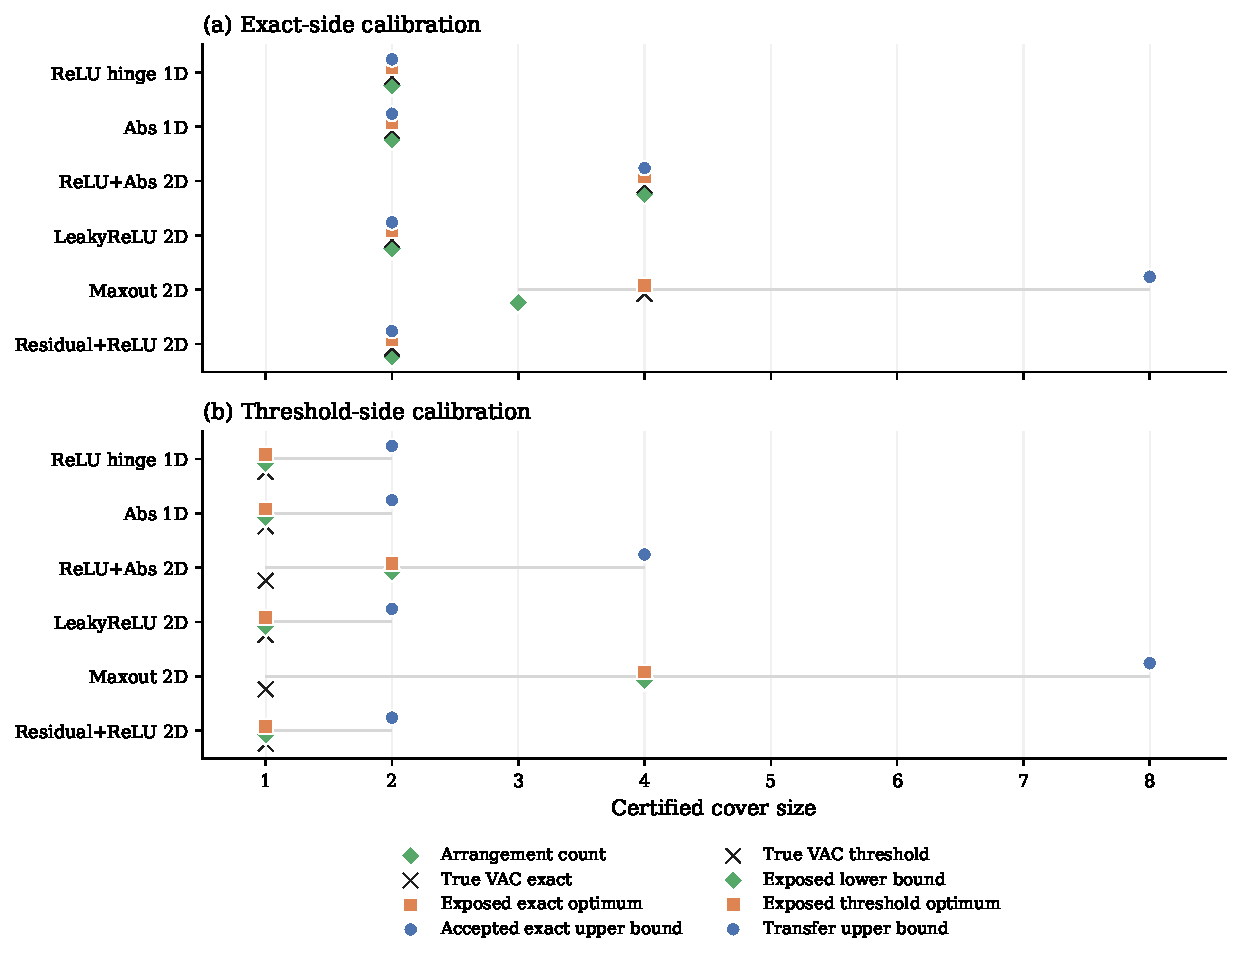
\includegraphics[width=0.94\textwidth]{figures/appendixI_goldtiny_calibration}
    \caption{Gold Tiny exhaustive calibration. Panel (a) compares arrangement count, true exact VAC in the guard language, the exposed exact optimum, and the accepted exactification upper bound. Five of the six tiny cases coincide on the exact side; the maxout case exhibits the intended separation \emph{arrangement count $<$ true exact VAC $<$ exactification upper bound}. Panel (b) compares true guard-language threshold VAC, the exposed lower bound, the exposed threshold optimum, and the transfer upper bound on canonical true-threshold tasks. This panel should be read as a language-calibration plot: exposed threshold quantities need not equal the true guard-language threshold VAC even on the tiny exhaustive suite.}
    \label{fig:appI-goldtiny-calibration}
\end{figure}

\clearpage
\subsection{Exact-Side Exactification and Compression}

Figure~\ref{fig:appI-exact-scaling} summarizes the constructive exactification upper bounds across the full benchmark suite. The accepted exact upper bound $U_{\mathrm{eq}}^{\mathrm{align}}$ grows with the number $H = |\mathcal H^\star|$ of compiled comparison hyperplanes, but on the saved bundle it stays well below the crude $2^H$ envelope. This is the main empirical counterpart of the finite exactification theorem: the theorem only guarantees a finite aligned split-tree upper bound, while the artifact shows that the realized upper bounds are much smaller than the coarsest combinatorial envelope on the benchmark families shipped here.

Figure~\ref{fig:appI-exact-compression} complements the scaling view with a compression view. The compression factor is
\[
\frac{U_{\mathrm{eq}}^{\mathrm{align}}}{\mathrm{OPT}_{\mathrm{eq}}^{\mathrm{exposed}}}.
\]
For Family A, Family B, and ThresholdStress, the median compression factor is $1.0\times$, meaning that the accepted exactification upper bound closely tracks the exposed exact optimum. Gold Tiny is also mostly at $1.0\times$, with the small maxout example producing the one visible exact-side gap. By contrast, SelectionStress is deliberately designed to enlarge the exposed candidate language while keeping the final semantic exact cover small, and the resulting median compression factor is $12.5\times$ with substantially larger outliers. This is the cleanest experimental manifestation of the paper's exact-side ``candidate exposure versus semantic optimum'' distinction.

\begin{figure}[t]
    \centering
    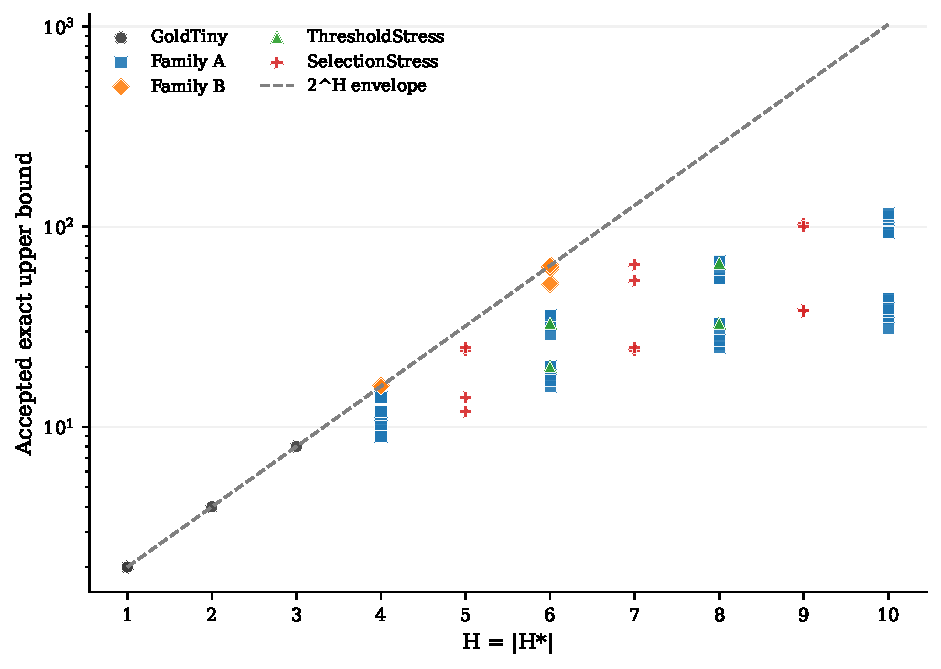
\includegraphics[width=0.78\textwidth]{figures/appendixI_exact_scaling}
    \caption{Exactification scaling across the full benchmark suite. Each point is one saved exact-side row. The dashed curve is the crude $2^H$ envelope. Accepted exact upper bounds grow with $H$, but remain far below the envelope on the shipped paper-facing bundle.}
    \label{fig:appI-exact-scaling}
\end{figure}

\begin{figure}[t]
    \centering
    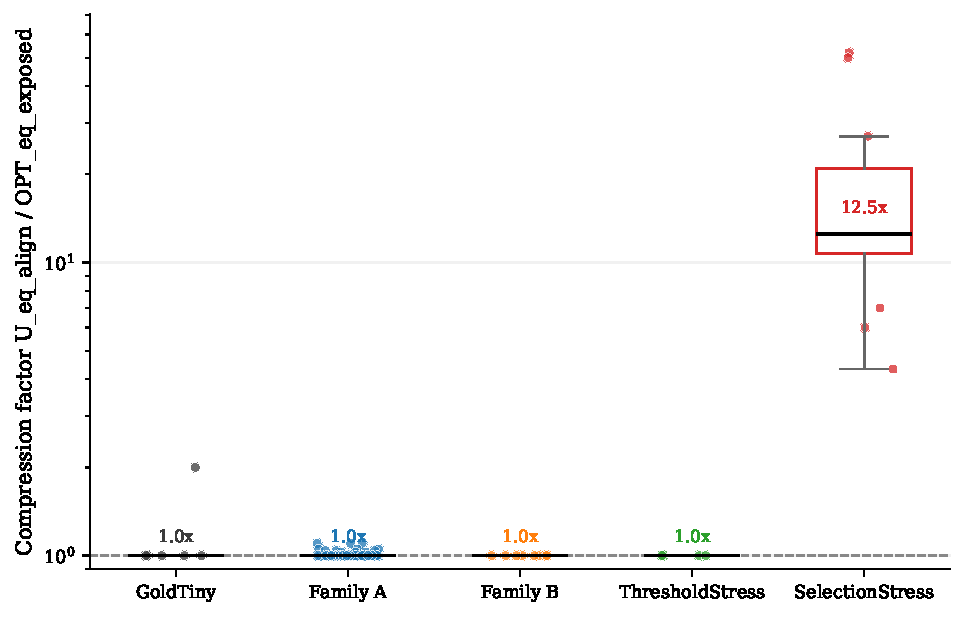
\includegraphics[width=0.80\textwidth]{figures/appendixI_exact_compression_by_family}
    \caption{Exact-side compression factor by family. The plotted quantity is $U_{\mathrm{eq}}^{\mathrm{align}} / \mathrm{OPT}_{\mathrm{eq}}^{\mathrm{exposed}}$. Family A, Family B, and ThresholdStress stay concentrated at $1.0\times$, while SelectionStress exhibits large exposed-language compression. Gold Tiny is almost entirely at $1.0\times$, with the maxout example providing the intended small deviation.}
    \label{fig:appI-exact-compression}
\end{figure}

\clearpage
\subsection{Threshold-Side Upper Bounds, Exposure, and Diagnostics}

The threshold side is organized around one canonical true-threshold task per instance together with one false control. The false controls are clean in the saved bundle: none of the 126 false-control rows admits a finite accepted threshold cover. On the positive side, Figure~\ref{fig:appI-threshold-gap} plots the transfer upper bound against the exposed threshold optimum for the canonical true tasks. Every point lies below the diagonal, exactly as expected from the transfer theorem: an accepted exact cover transfers to a threshold cover of no larger size.

The threshold story is more subtle than a blanket ``threshold is easier'' slogan. Figure~\ref{fig:appI-threshold-vs-exact} is included specifically to make that subtlety explicit. On Family A, Family B, Gold Tiny, and ThresholdStress, the exposed threshold optimum is typically below the exposed exact optimum. However, SelectionStress is intentionally a counterexample family: it targets exact-side cancellation/compression and therefore can have a much smaller exposed exact optimum while still requiring a larger threshold-side exposed cover in the bounded threshold language implemented by the artifact. The threshold section of the paper should therefore be written in the language-relative form used throughout the repository notes, not as a claim of universal threshold dominance.

Figure~\ref{fig:appI-threshold-stage} then isolates the threshold-stage exposure mechanism on the curated threshold subset. The conservative v3 default sets the parent-backtracking depth to zero, so the $D_{\mathrm{transfer}}$ and $+D_{\mathrm{parent}}$ stages are intentionally dormant controls. The visible gain arrives at the $+D_{\mathrm{drop}}$ stage: the median dictionary size increases from $38.0$ to $254.5$, while the median exposed threshold optimum decreases from $38.0$ to $19.5$. The median exposed lower bound stays at $16.0$, so the final stage is not merely adding vacuous candidates; it is exposing a strictly better cover language while remaining close to the certified lower-bound floor.

\begin{figure}[t]
    \centering
    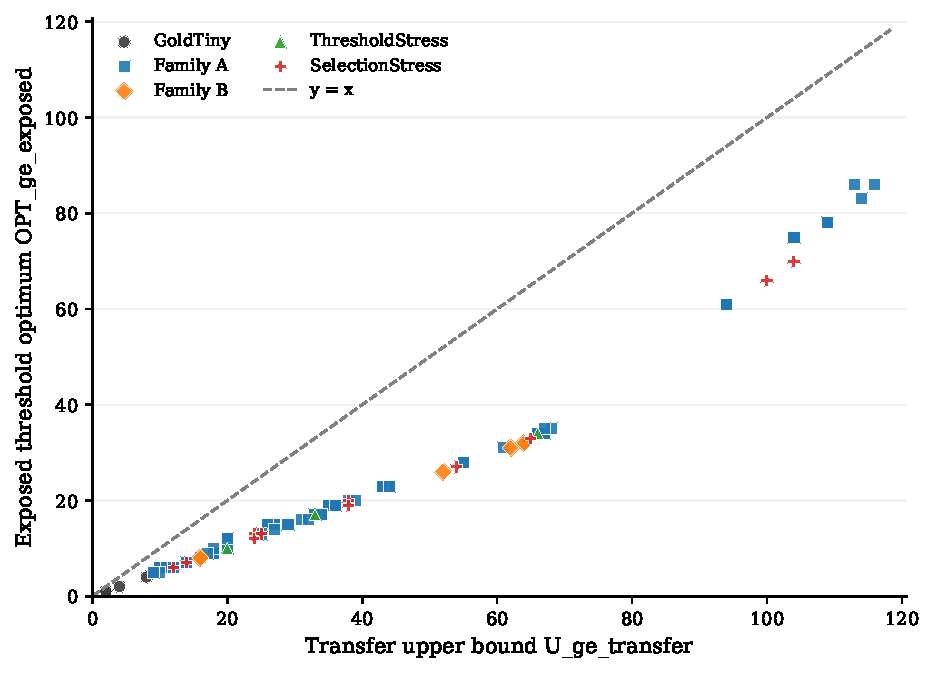
\includegraphics[width=0.80\textwidth]{figures/appendixI_threshold_transfer_gap}
    \caption{Transfer upper bound versus exposed threshold optimum on canonical true-threshold tasks. All points lie below the diagonal, as required by the exact-to-threshold transfer upper bound.}
    \label{fig:appI-threshold-gap}
\end{figure}

\begin{figure}[t]
    \centering
    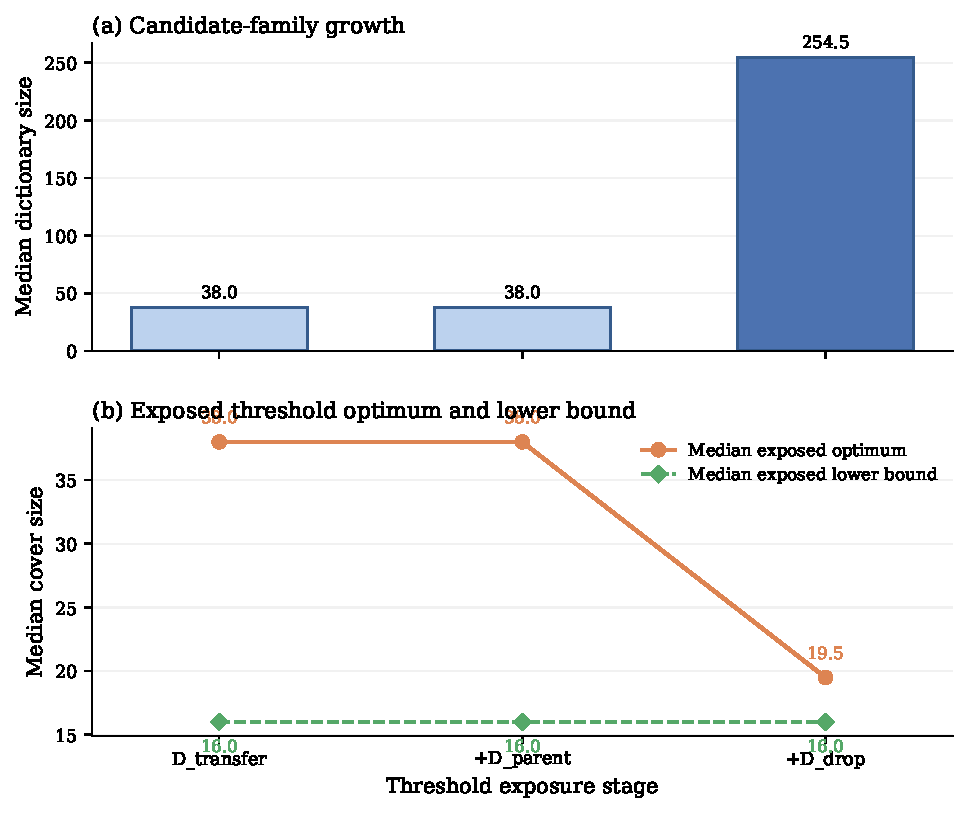
\includegraphics[width=0.80\textwidth]{figures/appendixI_threshold_stage_ablation}
    \caption{Threshold-stage ablation on the curated threshold subset. Under the conservative v3 default, parent backtracking is disabled, so $D_{\mathrm{transfer}}$ and $+D_{\mathrm{parent}}$ coincide. The $+D_{\mathrm{drop}}$ stage enlarges the exposed threshold dictionary and reduces the median exposed optimum from $38.0$ to $19.5$ while the median exposed lower bound remains at $16.0$.}
    \label{fig:appI-threshold-stage}
\end{figure}

\begin{figure}[t]
    \centering
    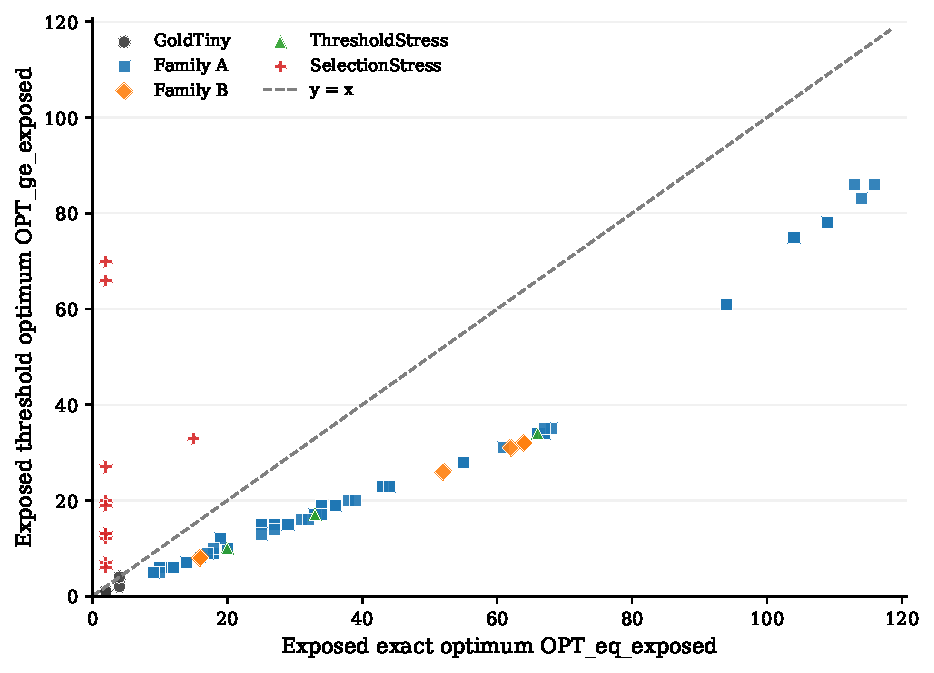
\includegraphics[width=0.80\textwidth]{figures/appendixI_threshold_vs_exact_diagnostic}
    \caption{Threshold-versus-exact diagnostic on the canonical true-threshold rows. Most benchmark families lie below the diagonal, while SelectionStress intentionally lies above it. Thus threshold exposed optima are not universally smaller than exact exposed optima; the comparison depends on the exposed candidate language and on the benchmark family.}
    \label{fig:appI-threshold-vs-exact}
\end{figure}

\clearpage
\subsection{Selection-Layer Exposure on Explicit Candidate Families}

The exact-side selection experiment is intentionally separated from the exactification scaling experiment. Its job is not to estimate unrestricted semantic hardness for every benchmark family. Its job is to show what happens after the pipeline has already exposed an explicit finite candidate family and the remaining problem is to select a smallest accepted subcover inside that family.

Figure~\ref{fig:appI-selection-stage} shows the stagewise behavior on the curated selection subset. The median dictionary size grows from $40.5$ at $D_{\mathrm{leaf}}$ to $145.0$ at $D_{\mathrm{leaf}} + D_{\mathrm{frag}}$, then to $224.0$ at $+D_{\mathrm{parent}}$, and finally to $586.0$ at $+D_{\mathrm{drop}}$. At the same time, the median exposed exact optimum stays at $40.5$ through the first two stages and then collapses to $3.0$ at the parent/drop stages. The qualitative lesson is that exposing more candidates can make the selection layer dramatically more informative before any theorem-level hardness statement is invoked.

The repository's SelectionStress family is deliberately targeted to make this phenomenon visible. Accordingly, Figure~\ref{fig:appI-selection-stage} should be interpreted as an explicit-dictionary stress demonstration rather than as a blanket empirical statement that selection is the dominant difficulty on every family. That scoped interpretation matches the theoretical hardness discussion in Section~\ref{sec:vac-minimization} and Appendix~\ref{app:dict-hardness}.

\begin{figure}[t]
    \centering
    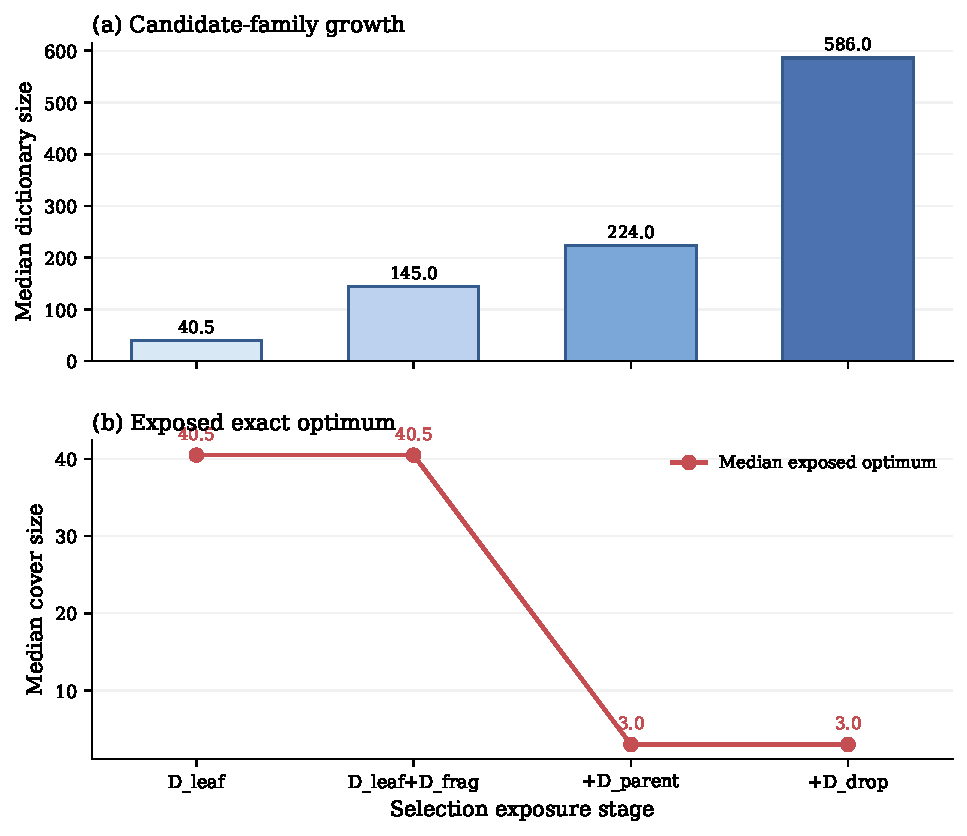
\includegraphics[width=0.80\textwidth]{figures/appendixI_selection_stage_ablation}
    \caption{Selection-stage ablation on the curated explicit-candidate subset. Candidate exposure grows from $D_{\mathrm{leaf}}$ to $+D_{\mathrm{drop}}$, while the median exposed exact optimum collapses from $40.5$ to $3.0$. This is a stress-family demonstration of selection-layer compression after candidate exposure, not a blanket claim about every benchmark family.}
    \label{fig:appI-selection-stage}
\end{figure}

\clearpage
\subsection{Realization-Side Payload, Checking Cost, and Runtime}

The realization figures separate the semantic proof payload from full engineering archives. This distinction is essential for interpreting the SCC/DL-facing part of the artifact. Figure~\ref{fig:appI-realization} shows that compact/core binary payload size is almost perfectly linear in proof-cell count, while archive bundles are much larger and vary strongly by family. On the saved bundle, the fitted core-byte slope is approximately $206$ bytes per proof cell, and the Pearson correlation between proof-cell count and compact/core binary size is about $0.995$. By contrast, the median archive-to-core ratio is only about $5.1\times$ on Gold Tiny but rises to roughly $21.6\times$ on Family A, $15.6\times$ on Family B, $18.5\times$ on ThresholdStress, and $251.7\times$ on SelectionStress. The archive should therefore be read as engineering overhead, not as a direct measure of semantic proof payload size.

Figure~\ref{fig:appI-core-check} shows the same near-linear behavior for checker runtime on compact/core payloads. The saved bundle stays below one millisecond for the core binary checker, with the largest observed values remaining around $0.6$ ms. Finally, Figure~\ref{fig:appI-generation-time} reports exactification generation time as a function of $H$. The paper-facing bundle is not designed as a maximal stress benchmark, yet it is still useful to record that the constructive exactification pass remains within a few seconds on all shipped instances. In the saved run, the largest generation times stay below approximately $6$ seconds.

Taken together, these figures support the main text's final empirical message: exactification yields observable finite exact covers with moderate constructive cost; threshold-side and selection-side exposure change the optimum before any hardness statement is applied; and compact/core proof realizations are the right object to compare at the realization layer, while full archive bundles should be reported separately.

\begin{figure}[t]
    \centering
    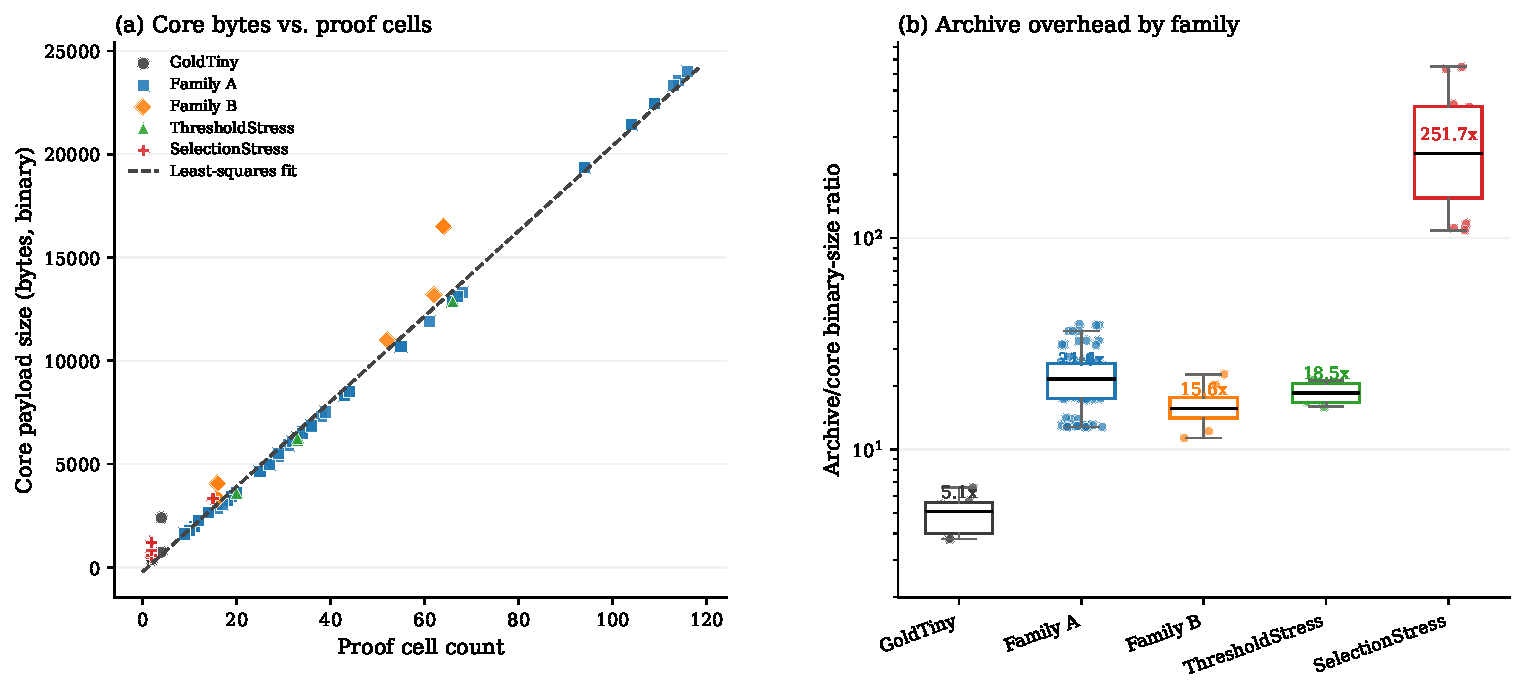
\includegraphics[width=\textwidth]{figures/appendixI_realization_dual}
    \caption{Realization-side payload metrics. Panel (a) shows near-linear scaling between proof-cell count and compact/core binary payload size. Panel (b) shows that archive bundles are much larger than compact/core payloads, especially on SelectionStress; archive size therefore should not be conflated with semantic proof payload size.}
    \label{fig:appI-realization}
\end{figure}

\begin{figure}[t]
    \centering
    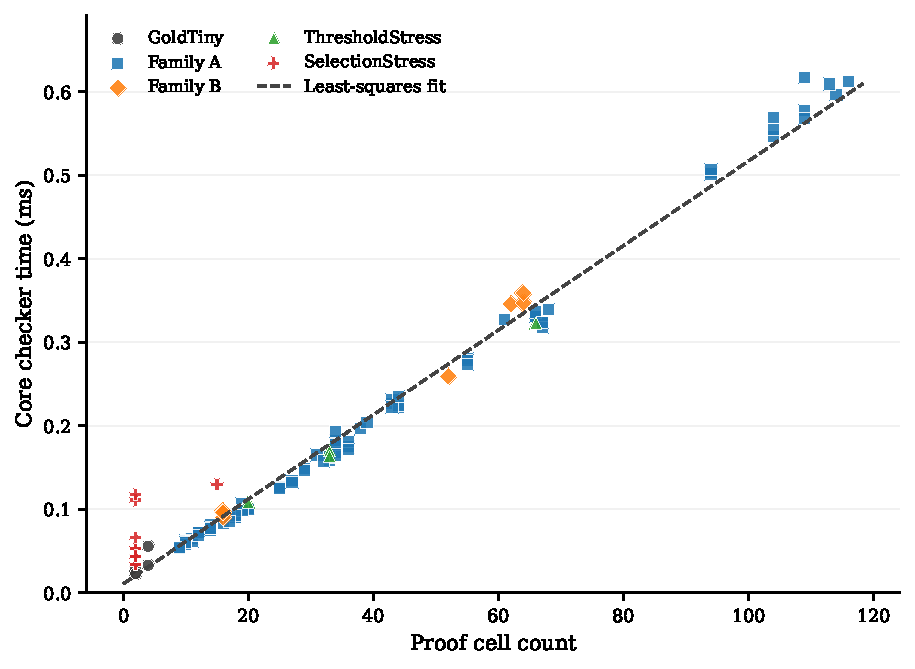
\includegraphics[width=0.80\textwidth]{figures/appendixI_core_checker_time}
    \caption{Compact/core checker time versus proof-cell count. Core checking remains sub-millisecond on the saved bundle and is close to linear in proof-cell count.}
    \label{fig:appI-core-check}
\end{figure}

\begin{figure}[t]
    \centering
    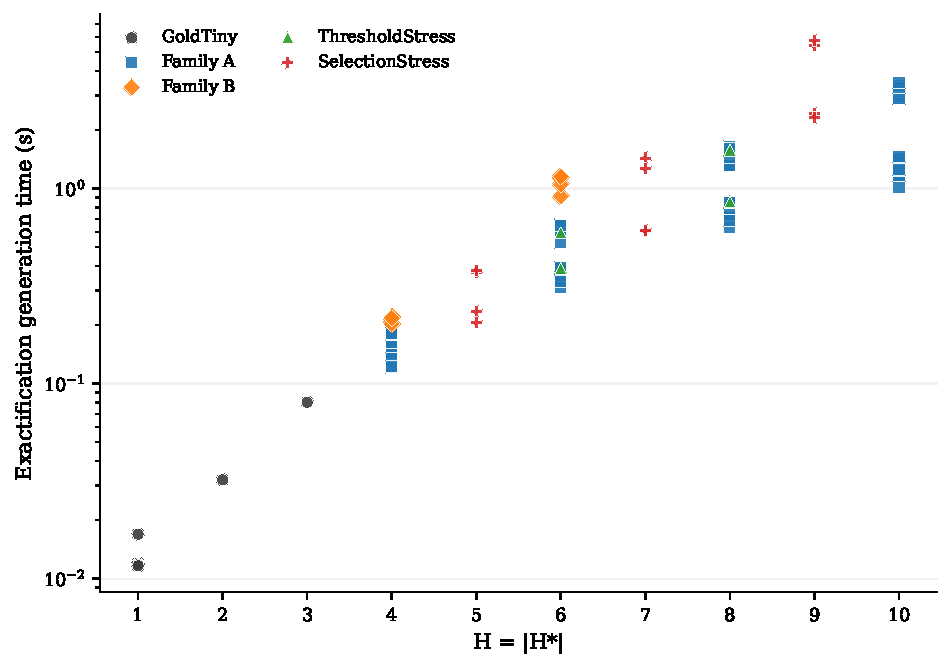
\includegraphics[width=0.80\textwidth]{figures/appendixI_generation_time}
    \caption{Exactification generation time versus $H = |\mathcal H^\star|$. The constructive exactification pass grows with problem size but remains within a few seconds on the saved paper-facing bundle.}
    \label{fig:appI-generation-time}
\end{figure}
